\section{Background of the Study}

Coffee is one of the most globally consumed beverages. It is a vital product in the global market, with production reaching 168.2 million bags in 2022-2023. The coffee industry is expected to grow even more in the coming years, with output projected to rise by 5.8% in 2023-2024 (International Coffee Organization, 2023). In the Philippines, coffee holds a strong cultural significance, with the local industry continuously expanding. The country is the 14th largest coffee producer in the world. Locally, the industry is expected to grow at a compound annual growth rate (CAGR) of 3.5% from 2021 to 2025, driven by small-scale farm households (Santos & Baltazar, 2022). With a growing popularity among coffee enthusiasts, the demand for specialty coffee is increasing as well. Consumers are becoming more selective about the quality of their coffee beans (Tampon, 2023).  

To stay competitive in the rapidly evolving coffee industry, farmers carefully select high-quality coffee beans for production. Grading green coffee beans is a crucial part of coffee production, as it is directly associated with the quality of the cup quality of coffee brews (Barbosa et al., 2019). Coffee grading is a process in the industry that determines the quality of coffee beans, using various parameters such as size, density, color, and defects, ensuring that only high quality beans are selected for consumption (Córdoba et al., 2021). The size of coffee beans is determined using a screen size and sorting procedure, where the coffee beans are categorized into different screen sizes, with larger beans considered higher quality (González et al., 2019). The density of a bean can be calculated by the ratio of its mass and volume, which greatly influences the roasting process and overall quality of the coffee (Datov \& Lin, 2019). Color is also another indicator for quality, with darker beans being preferred for their richer flavor profile. On the other hand, defects are classified among 3 categories: Category 1 includes the most severe issues such as foreign matter and black beans, Category 2 includes less severe defects like broken beans, and Category 3 includes minor defects like slight discoloration. Determining the quality of the coffee beans in relation to their defect values is based on quality standards and grading systems such as SCAA protocols guidance or the Philippine National Standard on Green Coffee Bean. 

Traditionally, this stage of assessing and categorizing coffee beans relies on visual evaluation, which is time-consuming and labor-intensive, making it prone to human error. One of the biggest challenges in coffee bean production is ensuring consistency in quality. As the demand for specialty coffee continues to grow, there has also been an increase for the need of more efficient and accurate sorting methods. The application of modern technology can help reduce the labor costs and minimize human errors in these tasks. In recent years, computer vision was used alongside various machine learning models and techniques, such as convolutional neural networks (CNNs), support vector machines (SVMs), or K-nearest neighors (KNN) models, where the models were trained on labeled data to classify images of coffee beans into different quality categories. The proposed aims to utilize this technology to develop a two-stage automated coffee bean sorting system using machine vision and density-based analysis to categorize and identify and segregate specialty-grade green coffee beans from non-specialty and defective coffee beans. 

\section{Prior Studies}
Identifying and sorting specialty-grade coffee beans can be strenuous since the traditional way of classifying a specialty-grade coffee is by manually sorting the coffee bean batch and classifying them according to the set of standards of the SCAA. The existing work aims to solve these problems through image processing and implementing deep learning-based models to automatically sort the coffee beans while achieving high accuracy. However, these solutions only automate detecting either one of the parameters such as defects, color, and size, while the proposed system considers density, size, color and defects all in one system. Hence, eliminating human intervention or labor. The table below shows the comparison of existing solutions to the researcher’s proposal aligning with the traditional way of sorting coffee beans. 

\begin{center}
    \begin{longtable}{| p{4cm} | p{10cm} |}
    \hline
    Existing Literature & Description \\ \hline
    Defect Detection & The existing literature focuses on using various machine learning models such as YOLO, KNN, and CNN to detect defects in green coffee beans, 
	through identifying visible defects like black spots, broken beans, discoloration, and more. These existing approaches heavily rely on visual characteristics 
	and do not consider other key factors that affect green coffee bean quality like density, which can enhance classification accuracy. The proposed system 
	integrates density and size analysis alongside the defecting various levels of defects on the coffee bean for a more holistic detection and classification. \\ \hline
    Coffee Bean Grading and Quality Assessment & The existing literature utilize algorithms such as artificial neural networks, support vector machine, and random 
	forest to grade and classify coffee beans according to the specified grading system. These methods primarily focus on visual features of the beans, 
	which do not account the bean’s density and size, which are both essential factors for classifying specialty-grade coffee beans. Additionally, there is a lack of 
	practical implementation of automated sorting systems, as these focus on simply classifying the beans. Through a two-stage process, the proposed system will 
	take into consideration both the visual inspection and the density measurement, which leads to a more complete classification of coffee beans. \\ \hline
    Automated Sorting and Classification System & Research has been conducted on developing that automate the process of sorting coffee beans according to various parameters. 
	Some studies focus on sorting defectives against non-defective, while others focus on other visual parameters like defects and roast profiles. These systems focus only on visual 
	characteristics, without considering the actual size of the bean and its density as parameters for better classification accuracy. The proposed system will integrate the use of visual, density, and size parameters to enable a comprehensive automated sorting solution for classifying specialty-grade coffee beans. \\
    \hline
    \end{longtable}
\end{center}

\begin{center}
	\small

    \begin{longtable}{| p{5cm} | p{4cm} | p{4cm} |}
    \hline
    Proposed System & Balay, D. D., Cabrera, R. M., Jensen, J. T. B., \& Mayuga, K. E. L. (2024). Automatic sorting of defective coffee beans through computer vision & A. J. N. Lualhati, J. B. Mariano, A. E. L. Torres, and S. D. Fenol, “Development and Testing of Green Coffee Bean Quality Sorter using Image Processing and Artificial Neural Network  \\ \hline
    
	\begin{itemize}
		\item Defect sorting using EfficientNetV2. 

		\item Considers classification of 10 defect types. 
	
		\item The system considers density parameters to sort out less-dense beans. 
	
		\item The system includes a graphical user interface for farmers to visualize the cumulative data of the defects present in the batch. 
	
		\item The system also includes AI-generated recommendations on the possible interventions for the farmers based on the data gathered from the sorting system.  
	\end{itemize}
	&
	\begin{itemize}
		\item Defect sorting using YOLOv8 

		\item The study considered only 6 types of defects. 
	\end{itemize}
	&
	\begin{itemize}
		\item Defect sorting using YOLOv2 and InceptionV3. 

		\item The study considered only 2 types of defects. 
	\end{itemize}
	\\
	\hline
    \end{longtable}
\end{center}

\section{Problem Statement}
The Philippine coffee industry is a growing market, however it is stuck with using traditional methods in sorting green coffee beans. Often relying on manually sorting the beans, it exposes a number of problems that are apparent in the industry. Relying on manual sorting increases production cost which results in higher prices for quality coffee beans. To make the Philippine coffee beans more competitive to the exported beans, reducing the price is crucial. Another problem that is encountered in manual sorting heavily focuses only on the physical attributes of the bean like size and appearance. There are standards that need to be met, which forces the farmers to resort to manual sorting to comply with the standards of the SCAA. The SCAA standards require a 300g batch of green coffee beans must not contain any defects and the size consistency of the beans must not exceed 5\% variance. Another reason why coffee processors still opt to do manual sorting is because there are no commercially available and reliable GCB sorting machines (Lualhati et al., 2022). There is a need for a coffee sorter that is able to efficiently and accurately sort GCB. Coffee bean selection is carried out either manually, which is a costly and unreliable process (Santos, 2020). The manual sorting process limits scalability and quality control, putting the strain on farmers as coffee shop owners' demands for high-quality coffee continue to rise (Lualhati et al., 2022).   	 	 

\section{Objectives and Deliverables}

Your objectives are the states that you desire to achieve in solving the problem. The general objective is the main state to be achieved whereas the specific ones are sub-states to be achieved.

\subsection{General Objective (GO)}
 \Copy{GO}{GO: To develop an automated (Arabica) green coffee bean sorter that identifies good, less-dense and defective beans from an unsorted batch of coffee beans. The system will utilize machine vision and density-based analysis for defect detection and classification of the coffee beans, ensuring efficient coffee bean sorting.};

\subsection{Specific Objectives (SOs)}

\begin{itemize}
	\item \Copy{SO1}{SO1: To gather and create a dataset consisting of 500 high-resolution images per classification of Arabica green coffee beans (dense, less-dense, defective (category 1 \& 2))};
	
	\item \Copy{SO2}{SO2: To improve the synchronization between the machine vision system and the embedded sorting mechanism, ensuring defect sorting of at least 20 beans per minute, solving issues such as non-synchronization of the system};
	
	\item \Copy{SO3}{SO3: To achieve an accuracy of at least 85\% in classifying defective green coffee beans using computer vision};
	
	\item \Copy{SO4}{SO4: To achieve an accuracy of at least 85\% in filtering out less-dense green coffee beans};
\end{itemize}



\subsection{Expected Deliverables}

Table~\ref{tab:expected_deliverables} shows the outputs, products, results, achievements, gains, realizations, and/or
yields of the \documentType. 


\begin{table}[!htbp]
	\caption{Expected Deliverables per Objective} 	
	\label{tab:expected_deliverables} 
	{\centering \scriptsize
		\begin{tabular}{p{0.2\textwidth}|p{0.7\textwidth}}
			\hline 
			\hline 
			\textbf{Objectives} & 
			\textbf{Expected Deliverables}\\ 
			\hline 
%%			\endfirsthead
%			\multicolumn{2}{c}%
%			{\textit{Continued from previous page}} \\
%			\hline
%			\hline 
%			\textbf{Objectives} & 
%			\textbf{Expected Deliverables}\\ 
%			\hline 
%%			\endhead
%			\hline 
%			\multicolumn{2}{r}{\textit{Continued on next page}} \\ 
%%			\endfoot
%			\hline 
%%			\endlastfoot
%			\hline							

			\Paste{GO} & A Two-Stage Automated Coffee Bean Sorter System that identifies defective, good beans, and less-dense green coffee bean using machine vision and density-based analysis.  \\ \hline

			\Paste{SO1} & \begin{itemize}
				\item Data Gathering 

				\item Image Collection through High Quality Camera 
			\end{itemize} 
			\\ \hline		
%
			\Paste{SO2} & \begin{itemize}
				\item Improving the synchronization of machine vision and embedded sorting mechanism of the system.
			\end{itemize} 
			\\ \hline
%						
			\Paste{SO3} & \begin{itemize}
				\item Computer Vision Program 
				\item Sorting Mechanism 
			\end{itemize} 
			\\ \hline
%						
			\Paste{SO4} & \begin{itemize}
				\item Density-based Analysis 
				\item Sorting Mechanism 
			\end{itemize} 
		 	\\ \hline
%						
%			
		\end{tabular}
	}
\end{table}



\section{Significance of the Study}

The study explores the implementation of machine Vision and density analysis of an automated coffee been sorter that can identify and sort out the defective, less-dense and good green coffee beans. This said system would aid coffee sorters to mitigate manual labor and to ensure that the sorting process of the GCB are accurate. In order to test the effectiveness of the system, the study would gather data and compare the time efficiency and accuracy of the manual sorting by a an expert sorter to be compared with the proposed system. The system proposes significance to specific parts of society as follows: 

\subsection{Technical Benefit}

This study would benefit the academe as this introduces a significant advancement in coffee bean sorting technology by implementing both machine vision and density-based analysis to detect and sort good coffee beans, less-dense and separating defective ones. The proposed system would mitigate manual sorting that leads into insufficency like human error and fatigue. The system would improve the overall efficiency by operating at a faster rate compared to manual labor. As a result, it would serve as a proof of concept for the implementation of machine vision and  density-based analysis in agricultural  industries specifically in the Philippine coffee industry. 

\subsection{Impact to the Coffee Industry}

The study would aid coffee farmers and producers, by providing an automated system that ensures accurate sorting of Arabica green coffee beans, the system aims to have an accurate output to help maintain to yield higher quality coffee beans and allows coffee bussinesses to scale up their operations, increase the competitiveness of  exporting those beans, and meet demand more efficiently. The productivity given from the system would potentially strengthen the foundation of local coffee producers.  

\section{Assumptions, Scope, and Delimitations}

\subsection{Assumptions}

\begin{enumerate}
	\item There would be a defective coffee bean from the green coffee bean test batch;
	
	\item Identifying the defective coffee beans using the machine vision and density-based analysis would be much more efficient and accurate than manually sorting them;
	
	\item During testing, test batches will contain 50\% good beans and 50\% defective beans, 60\% good beans and 40\% defective beans, 70\% good beans and 30\% defective beans, 80\% good beans and 20\% defective beans, 90\% good beans and 10\% defective beans, 100\% good beans;	
\end{enumerate}

\subsection{Scope}
\begin{enumerate}
	\item The study only focuses on Arabica green coffee beans;
	
	\item The study has two stages, the first stage would segregate the defective green coffee beans from the batch, then the second stage would identify the specialty-grade green coffee beans depending on its density;
\end{enumerate}

\subsection{Delimitations}
\begin{enumerate}
	\item The batch of coffee beans to be used for testing and dataset collection will consist solely of Arabica beans from the same origin, farmer, and processed in the same way;
	
	\item The system is only limited to unroasted green coffee beans;
	
	\item The batch of coffee beans to be used should only be dehulled and not sorted visually and by density;

	\item Since the system is considering several types of defects and density parameter, sorting time is compromised;

	\item The system is designed to perform individual scanning of each coffee bean;
\end{enumerate}

\section{Description and Methodology of the \documentType}
\subsection{Manual Sorting}
\begin{center}
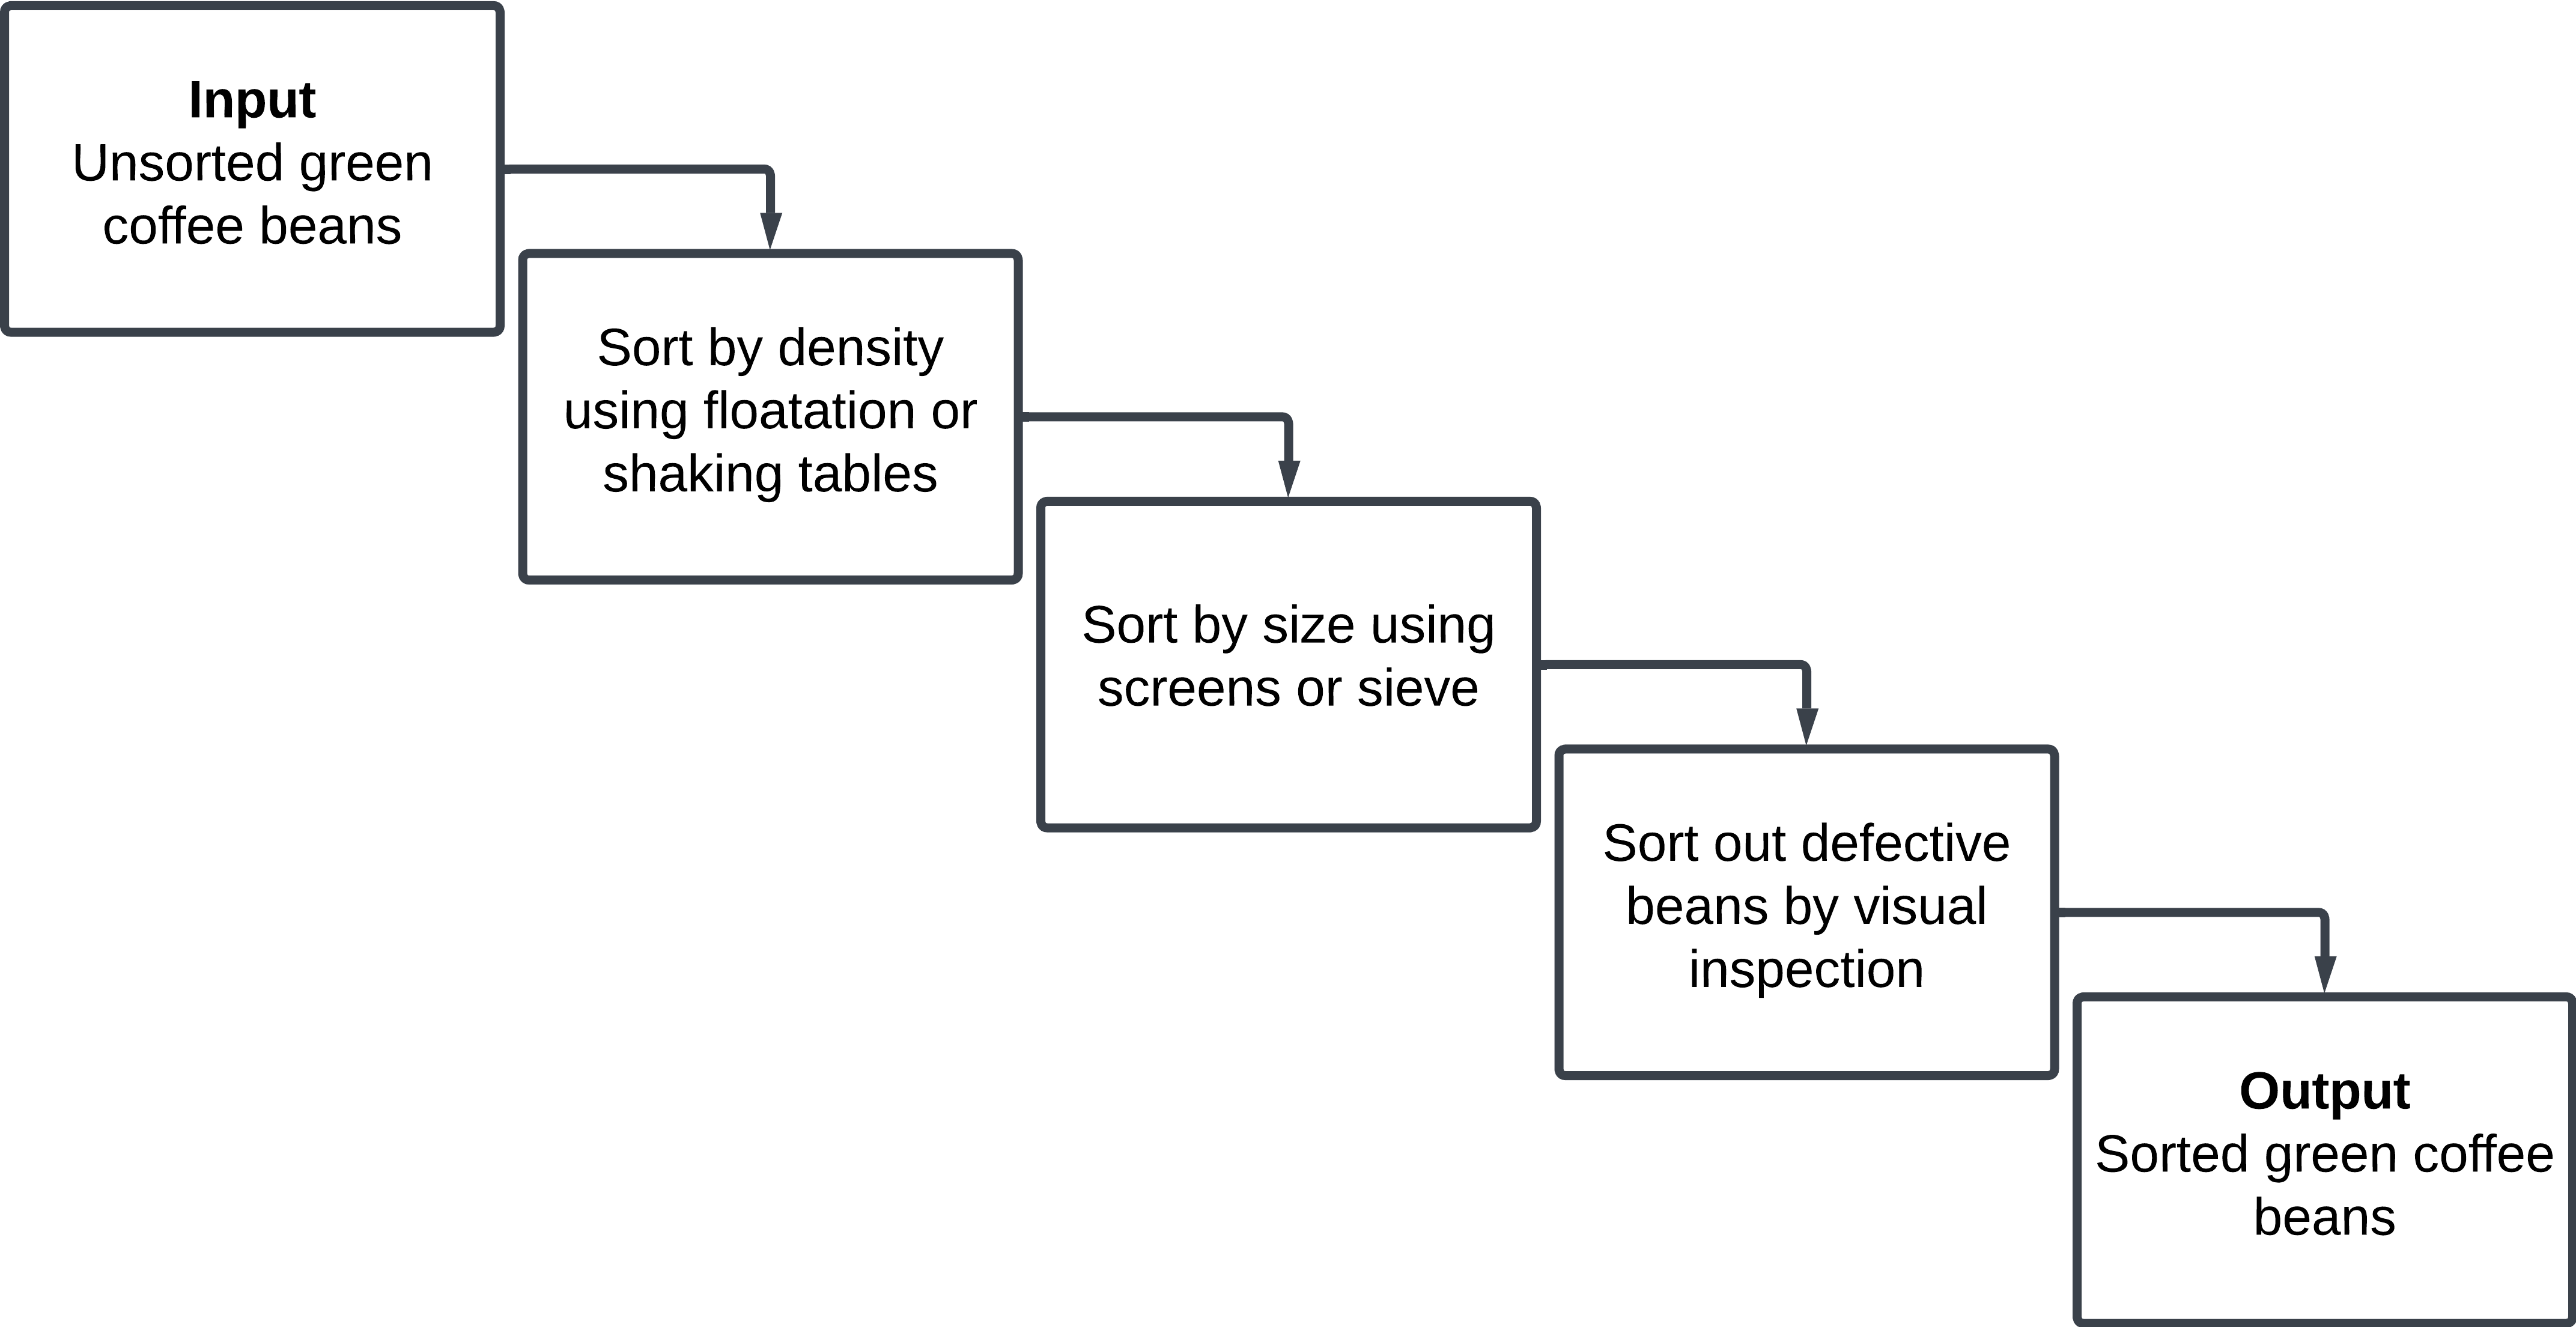
\includegraphics[width=0.9\textwidth]{figure/manual_sorting.png} 
\end{center}

The diagram in Figure 1 depicts the representation of the process of manual sorting of unsorted green coffee beans through a series of steps. First, the beans are sorted by density using methods such as floatation or shaking tables. This helps in separating the denser beans, usually pertaining to a more developed and higher quality bean. Then, the beans are sorted by size using screens and sieves with specific dimensions depending on the variety of the beans. After this, a thorough visual inspection is performed by the sorters to identify and remove the defective beans from the batch. The visual inspection includes sorting out cracks, discoloration, undeveloped and other defective bean characteristics. Finally, the process results in the output of sorted green coffee beans, ready for further processing or sale. 

\subsection{Description of the System}

\includegraphics[width=0.9\textwidth]{figure/placeholder.png} 

The proposed system is a two-staged automated green coffeee bean sorting machine, integrating both machine vision and density analysis. Firstly, the coffee beans are introduced into the system through a funnel, which directs them to a conveyor belt mechanism.  In the first stage, the green coffee beans will be sorted depending on their visual characteristics. In this stage, the physical qualities of the bean is analyzed such as size, color, and defect. If the bean is defective, the system will automatically sort it out. Then, all the non-defective beans will go through the second stage of the system. In the second stage, there will be an IR sensor and a weighing scale. The IR sensor will help the system to calculate for the estimated volume of the bean. The volume and mass of the bean in hand, the density of the bean can be calculated. Depending on the density threshold and size threshold set by the user, the bean will be classified whether it is good or not.


\includegraphics[width=0.9\textwidth]{figure/placeholder.png} 

Figure 3 shows the schematic diagram of the proposed system. Arduino Uno microcontroller magaes all the mechanical components such as the servo motor, stepper motors, and the converyor belt. The servo motor controls the  roitating mechanism for bean sorting. On the other hand, the stepper motors operate a slide mechanism to direct the beans. Two cameras, integrated with OpenCV via Python, handle machine vision algorithms, and image processing for defect detection of the beans. A ToF10120 sensor provides precise distance measurement. A precision weighing scale measures the density of each bean for classification. The Arduino communicates with the OpenCV system through serial communication, ensuring smooth coordination.


\includegraphics[width=0.9\textwidth]{figure/placeholder.png} 

Figure 4 shows the design overview of the system. Beans are first arranged through a hopper and a conveyor belt. On top of the conveyor belt, a 3D-printed guide is attached for the beans to maintain a linear formation. Then, the beans are expected to fall into another funnel attached to a tube. The tube is directly attached to a rotating mechanism that allows the beans to be inspected and sorted one-by-one. In this stage, defective beans are sorted out. Then, the non-defective beans are transferred onto the precision scale to analyze the density. The less-dense beans are sorted out of the batch.


\includegraphics[width=0.9\textwidth]{figure/placeholder.png} 

\subsection{Dataset and Model Training}
For the dataset collection, Arabica specialty-grade green beans from a farm will be used. Each bean is expected to be captured by a high-resolution camera with sufficient lighting. The top and bottom side pictures of the beans are to be collected. In addition, defective beans of the same type and origin will be gathered to identify the different classification of defects (primary and secondary). In this study, all primary defects are considered such as Full Black, Full Sour, Dried Cherry, Fungus Damage, and Severe Insect Damage. On the other hand, secondary defects are also considered such as Partial Black, Parchment, Floater, Shell, and Chipped. For the dataset collection, at least 500 images of good beans and at least 200 beans for each defect classification will be gathered to train the model. To further improve and increaase the dataset size, augmentation will be applied by scaling, rotating, and mirroring the images. 

The models to be used in this study are Convolutional Neural Network (CNN) and Random Forest. The CNN model is mostly compatible for image classification and feature extraction as it is composed of several different layers resulting in a better representation of image data (Wang et al., 2021). Thus, this model is the most ideal for green bean defect detection by identifying its texture, color, size, volume, deformations, and cracks in the first stage of sorting. Then, for the second stage where density parameter is added, Random Forest will be used. Since mixed data types are being considered (visual features extracted by CNN and density values), Random Forest is the best fit for this classification (Rigatti, 2017). In addition, the model is robust to overfitting, which means that it can handle noisy data. 

\subsection{Testing}
For the testing procedures, processed but unsorted green coffee beans will be acquired from a local farmer. These coffee beans will be sorted manually based on their different defects and quality, and also will be fed into the automated system to compare accuracy and performance. In line with the Philippine National Standard  or PNS (2022) for testing green coffee bean sorters, three test trials will be conducted. These trials will be conducted under similar operational settinsg to ensure consistency. The duration of each trial begins when the beans are fed into the system’s hopper and endsd after no beans remain in the system. During these trials, the system’s ability to sort defective beans and categorize the good beans by density will be monitored.
To create the dataset, coffee beans will be arranged on a sheet of paper and photo of the entire sheet will be taken. A program using YOLOv8 will then be used to process this image, detecting each bean, creating bounding boxes, and crop them into separate image files for labeling. Additionally, an alternative method involves using the system itself to collect data, with cameras capturing the top and bottom of the beans as they pass through the system. These approaches aim to ensure to create a diverse dataset that will be used for training the machine learning model.

In evaluating the system’s performance, various metrics, as dictated by the PNS for Green Coffee Bean Sorters, will be considered: 
\begin{itemize}
	\item \textbf{Sorting Accuracy}. The system’s sorting accuracy will be verified by comparing the output of the system to the manually sorted output of the same batch of beans.
	\item \textbf{Duration of Tests}. The total operating time for each trial will be recorded.
	\item \textbf{Sorting Yield}. The quantity and quality of the beans sorted in each trial will be measured to assess the system.
\end{itemize}


The desired accuracy of the system for its defect sorting is an accuracy of at least 85\%. The paper of Lualhati et al. (2022) was able to achieve an accuracy score of 85\% for sorting out good beans and 95\% for defect sorting, with an average score of 90\% for sorting out both. However, their paper only included two types of defects (black and deformed), and good quality beans as its data set. This study aims to target 10 types of defects along with the good green coffee beans ensuring that the system can cover a wider range of defects while also matching the accuracy of the previous study. 

To validate the performance of the system, the results will be compared with those obtained during the manual sorting. This comparison will focus on determining the accuracy of the defect detection and bean classification. The manual sorting process will serve as the reference for evaluating the system’s ability to enhance sorting efficiency and accuracy.

\subsection{Graphical User Interface (GUI)}
The proposed system would be integrating a graphical user interface developed using PyGui and ChatGPT API. The GUI would serve as the control center platform for the system. This would provide real-time feedback and insights for users. As shown in Figure 8, a concept of how the GUI would interact with the system would be a start button, once the button is executed the system would then be expecting inputs and start sorting. There would be real-time feedback during the sorting process, then some visual markers to indicate their classification, and an elapsed time so the user would be aware of the time of the sorting process. Once the system is done, the user can click the end button and the summary report would generate in an orderly manner, providing tables of classification that was detected through the process. In the bottom part of the GUI, ChatGPT API would be integrated and would offer recommendations based on the detected quality and classification of the coffee beans. 

\ifFinished
\else

\section{Estimated Work Schedule and Budget}

The estimated work schedule can be represented as a Gantt Chart or a combination of Project Network Diagram, Work Breakdown Structure, and Critical Path.  The budget can be made into a Bill of Materials, financial plan, or if your \documentType \ is funded and part of larger project, the cost, and date for reaching each milestone and/or deliverable for your part of the project.

For ECE Department undergraduate theses, the individual Gantt Chart or Work Breakdown Schedule and Bill of Materials will be included in this section and be removed in the final document.

\graytx{\blindtext}

\ifPhD
\section{Publication Plan}
\graytx{\blindtext}
\fi

\fi


\section{Overview of the \documentType}

Provide here a brief summary and what the reader should expect from each succeeding chapter.  Show how each chapter is connected with each other.

